\documentclass{article}
\usepackage[margin=24mm]{geometry}
\usepackage{tikz}
\title{Reverse jet: joint state and phase schedules}
\date{Created-at: 2026-10-29 01:22 CET}
\begin{document}\maketitle
\paragraph{Acceptance and scope.} Compare bounded phase-correct schedules for
the reverse 24-bit Hermite jet, then screen their full-context costs. Preserve
the existing 883-qubit incumbent. Admit a full 102400-shot official run only
after small native checks and a promising integrated resource screen. A negative
screen is recorded, not silently converted into a claimed score improvement.
\paragraph{Ownership.} Quantum owns a typed Core recipe, immutable native
composition, phase-contraction lowering, and verification. Existing Core/Query,
Graph/SBSH/P-graph selection and external Apache arithmetic stay with their
owners. No new parser, IR, matroid solver, dependency or provider modification.
\paragraph{Candidates.} Retained-cache reference; release the six-bit inverse
norm during scaling and recompute it for phase erasure; use the faster cached
inverse in a direct reverse with immediate old-v phase repayment; additionally
retain the exact zero flag into a contracted inverse phase. Compare public and
own fresh scalar inverses where compatible. Maximum eight recipes and twelve
pair checks, three seeds and 2048 probes per seed. Identify dominated schedules
and the actual peak allocation, including unchanged decoder stages.
\paragraph{Phase contract.} The held-flag inverse phase consumes F=[x=0].
Factor the phase via the two tower norms. Transpose the GF64 product tensor to
compute the six-bit quantum coefficient, use the existing held-flag inverse
phase, then measure the coefficient and repay its quadratic phase. Independently
check field-inverse phase for zero, basis, random inputs and random masks.
Retiring a cache must preserve its later consumers or charge recomputation.
\paragraph{Files and interfaces.} Extend synthesis.rs/NativeRecipe and native
metadata with a bounded Hermite-jet recipe; add source fixtures and direct tests.
Extend hermite.py and its CLI/tests with composition, phase checks and allocation
traces. Extend report.py for the campaign, and the existing native recipe/portfolio
workflow for Core selection. Add report data and this plan. Protected items: none.
\paragraph{Verification.} Fresh fetch succeeded; branch feat/unversioned at
32c6bb3 is current with upstream. Preserve existing dirty work. Targeted synthesis
and Python tests; native reference/own cross pairs; no phase cancellation accepted
from roundtrip alone. Serialize/reload candidate jet circuits. Matroid and P-graph
claims are limited to existing checked components and bounded portfolio selection.
\paragraph{Budget and ETA.} About 45--60 minutes after discovery, including
implementation, native cells, report and archive. Amaterasu has 317 GiB free.
One CPU, 2 GiB hard / 1800 MiB sampled memory, 900 seconds per small cell; an
admitted full build/verify may use 12 GiB and 900 seconds. Use existing runtime
and public-source mounts, current Python over stdin; no copied remote tree or WSL.
\paragraph{Risks and rollback.} Classical-mask and quantum-mask contractions
have different Toffoli cost. A smaller cache may require expensive recomputation.
Joint phase errors can hide in self-pairs, so use independent phase oracles and
cross-pairs. Narrowing one stage need not lower the global peak. Keep old artifacts;
roll back only task edits, never unrelated changes. No commit, push or submission.
\begin{center}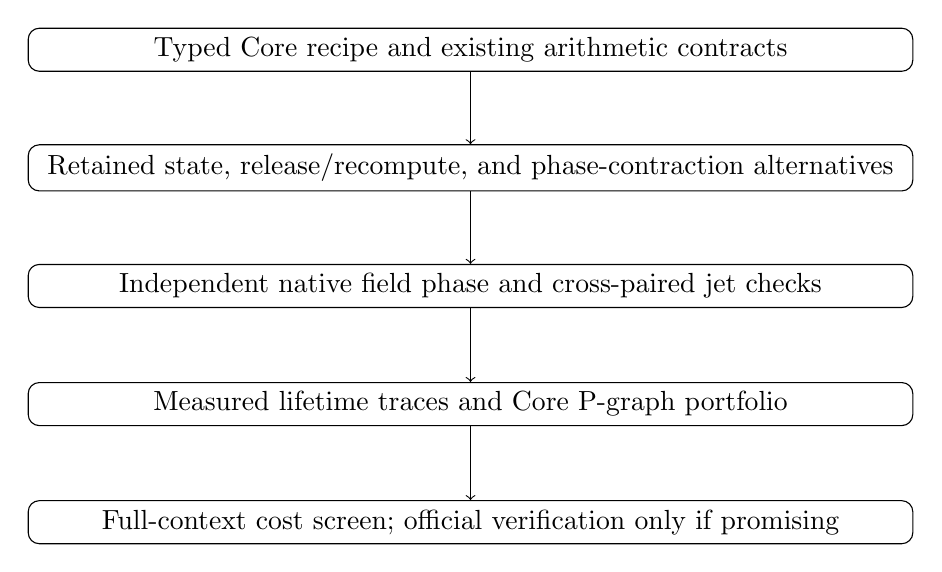
\begin{tikzpicture}[every node/.style={draw,rounded corners,align=center,text width=11cm},node distance=15mm]
\node (a) {Typed Core recipe and existing arithmetic contracts};
\node (b) [below of=a] {Retained state, release/recompute, and phase-contraction alternatives};
\node (c) [below of=b] {Independent native field phase and cross-paired jet checks};
\node (d) [below of=c] {Measured lifetime traces and Core P-graph portfolio};
\node (e) [below of=d] {Full-context cost screen; official verification only if promising};
\draw[->] (a)--(b);\draw[->] (b)--(c);\draw[->] (c)--(d);\draw[->] (d)--(e);
\end{tikzpicture}
\end{center}
\end{document}
